\chapter{Implementacja}
\label{cha:implementacja}
%Możliwości wyboru technologii dla rozwiązania problemu omawianego w~niniejszej pracy jest bardzo wiele. Począwszy od popularnych języków obiektowych jak Java, która swoimi, niemal nieograniczonymi możliwościami i~ogromem rozszerzających je bibliotek, pozwala rozwiązywać dowolne problemy czy technologii webowych jak JavaScript, która  

Praktyczna część niniejszej pracy została zrealizowana w~środowisku Matlab 2015b (darmowa wersja próbna). Łączy on niemal wszystkie kwestie poruszane w~niniejszej pracy - zaawansowane obliczenia matematyczne, przetwarzanie zbioru danych, pozwala na dynamiczne budowanie wykresów do prezentacji. Sprawdza się idealnie w~przypadku zadań analitycznych bądź symulacyjnych, a~jego konfiguracja sprowadza się do instalacji samego programu. Triangulację przeprowadzono w~oparciu o~klasę \textit{delaunayTriangulation}.

\section{Konwersja współrzędnych geograficznych}
Współrzędne poszczególnych punktów wejściowych określane są poprzez współrzędne geograficzne w~formacie dziesiętnym. Wobec tego, konieczne jest przekształcenie ich na wartości metryczne, aby móc wyznaczyć wartość opadu w~jednostkach SI.

Jednostki wzdłuż osi $Y$ przekształcone zostały stosując zależność $1^o=111196.672 [m]$, ponieważ w~przypadku szerokości geograficznej jest ona stała.

Dla długości geograficznej sytuacja nie jest tak prosta, gdyż długość jednego stopnia zależy od równoleżnika, na którym dokonuje się pomiaru. Przyjęto, że konwersja zostanie przeprowadzona w~oparciu o~długość równoleżnika leżącego na średniej szerokości geograficznej danych wejściowych. Praca zorientowana jest na analizę opadu z~konkretnej zlewni, zatem różnica z~wartością rzeczywistą jest niewielka (zostanie podana dla konkretnego przypadku). Przekształcenia dokonano w~oparciu o~wzór~\ref{eq:konwersja_wspolrzednych}. Do obliczeń przyjęto promień równikowy Ziemi o~wartości 6378410~m.

\begin{equation}
	r = \cos(\alpha)*R \Rightarrow 1^o = \frac{2 \pi r}{360} [m] \\
	\label{eq:konwersja_wspolrzednych}
\end{equation}
gdzie
\begin{description}[leftmargin=2cm, itemsep=0cm, labelsep=0cm]
	\item[$\alpha$] kąt, będący wartością szerokości geograficznej,
	\item[$R$] równikowy promień Ziemi,
	\item[$r$] promień równoleżnika na szerokości geograficznej $\alpha$.
\end{description}


\begin{figure}[!ht]
	\centering
	\includegraphics[width=0.3\linewidth]{ziemia}
	\caption{Schemat dla konwersji współrzędnych geograficznych.}
	\label{fig:ziemia}
\end{figure}

\section{Wielkość opadu}
\label{sec:funkcje_opadu}
Z~powodu braku dostępu do rzeczywistych danych meteorologicznych oraz hydrologicznych, co zostało opisane w~rozdziale~\ref{cha:odczyt_danych}, wykluczona została możliwość racjonalnej i~miarodajnej analizy pomiarów wraz z~określeniem korelacji opadu i~wysokości poziomu wody rzeki. Wobec powyższego, zdecydowano o~zastosowaniu danych symulowanych. Stworzone zostały funkcje generujące pomiar opadu we wskazanym punkcie. Przygotowane zostały dwa warianty - opad paraboliczny oparty na wzorze~\ref{eq:opad_parabola} oraz zdefiniowany funkcją wymierną~\ref{eq:opad_wymierny}.


Pierwszy z~nich jest funkcją wklęsłą. Należy zaznaczyć, iż zastosowanie jej do generowania wartości opadu wymaga spłaszczenia, gdyż interesujące są jedynie wartości większe lub równe 0. Dla tego przypadku spodziewa się wyniku z~niedomiarem w~stosunku do wartości rzeczywistej. Drugi jest bardziej zróżnicowany. Posiada obszary wklęsłe i wypukłe. Spodziewany wynik powinien być bardziej dokładny. Zastosowanie wyżej opisanych metod pozwoli na weryfikację działania programu w~odmiennych warunkach.

\begin{equation}
z = h \cdot (1 - (\alpha (x - x_0)^2 - \beta (y - y_0)^2) );
\label{eq:opad_parabola}
\end{equation}
gdzie
\begin{description}[leftmargin=3cm, itemsep=0cm, labelsep=0cm]
	\item[$\alpha, \beta$] współczynniki modyfikujące kształt opadu,
	\item[$x_0, y_0$] współrzędne środka płaszczyzny,
	\item[$h$] maksymalna wartość opadu.
\end{description}

\begin{equation}
z = h \cdot \frac{1}{1 + \alpha (x-x_0)^2 + \beta (y-y_0)^2}
\label{eq:opad_wymierny}
\end{equation}
gdzie
\begin{description}[leftmargin=3cm, itemsep=0cm, labelsep=0cm]
	\item[$\alpha, \beta$] współczynniki modyfikujące kształt opadu,
	\item[$x_0, y_0$] współrzędne środka płaszczyzny,
	\item[$h$] maksymalna wartość opadu.
\end{description}

Ustalona na potrzeby przeprowadzonych testów wielkość maksymalnego opadu wynosi 100 milimetrów. Dla opadu parabolicznego przyjęto współczynniki $\alpha$ i $\beta$ o wartościach odpowiednio \num{50e-12} oraz \num{70e-12}, natomiast dla drugiego wariantu opadu \num{50e-12} i~\num{200e-12}. Kształt funkcji opadu przedstawiają rysunki~\ref{fig:opad_paraboliczny} oraz~\ref{eq:opad_wymierny}.

\begin{figure}[!ht]
\centering
	\begin{subfigure}{1\textwidth}
		\centering
		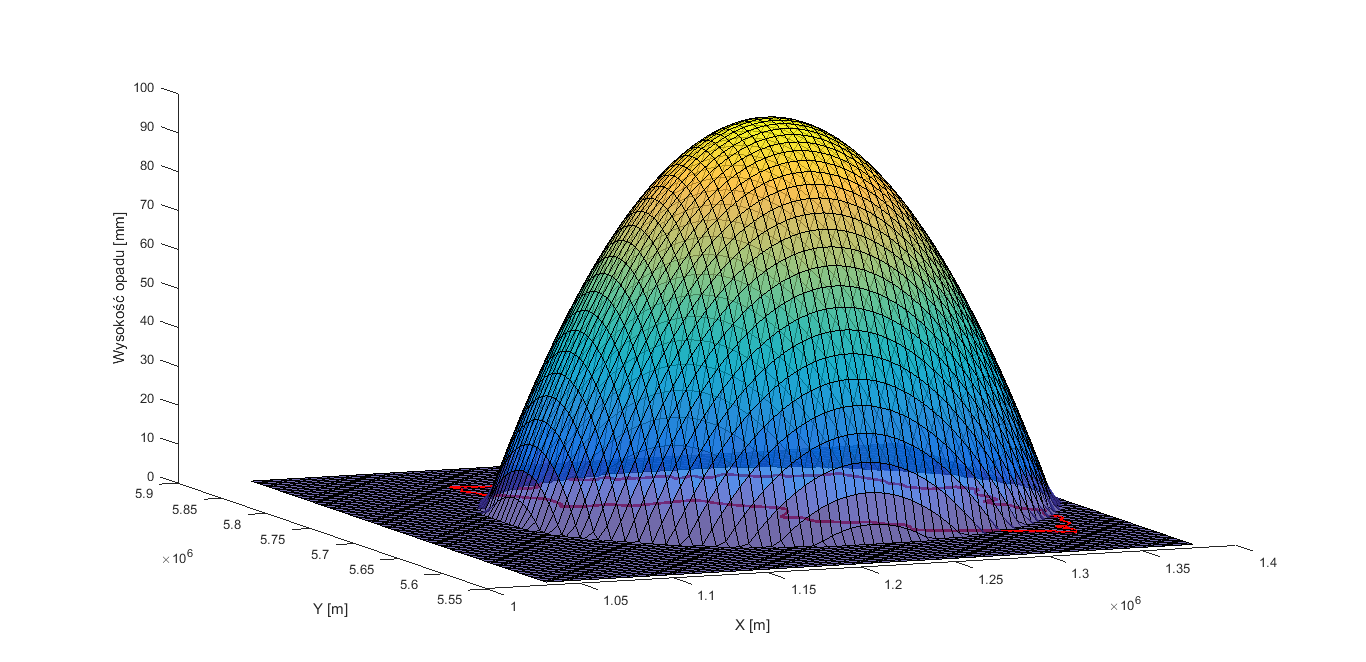
\includegraphics[width=1\linewidth]{chmura_paraboloidalna_1}
		\caption{Wykres trójwymiarowy.}
		\label{fig:parabola_3d}
	\end{subfigure}	
	\begin{subfigure}{1\textwidth}
		\centering
		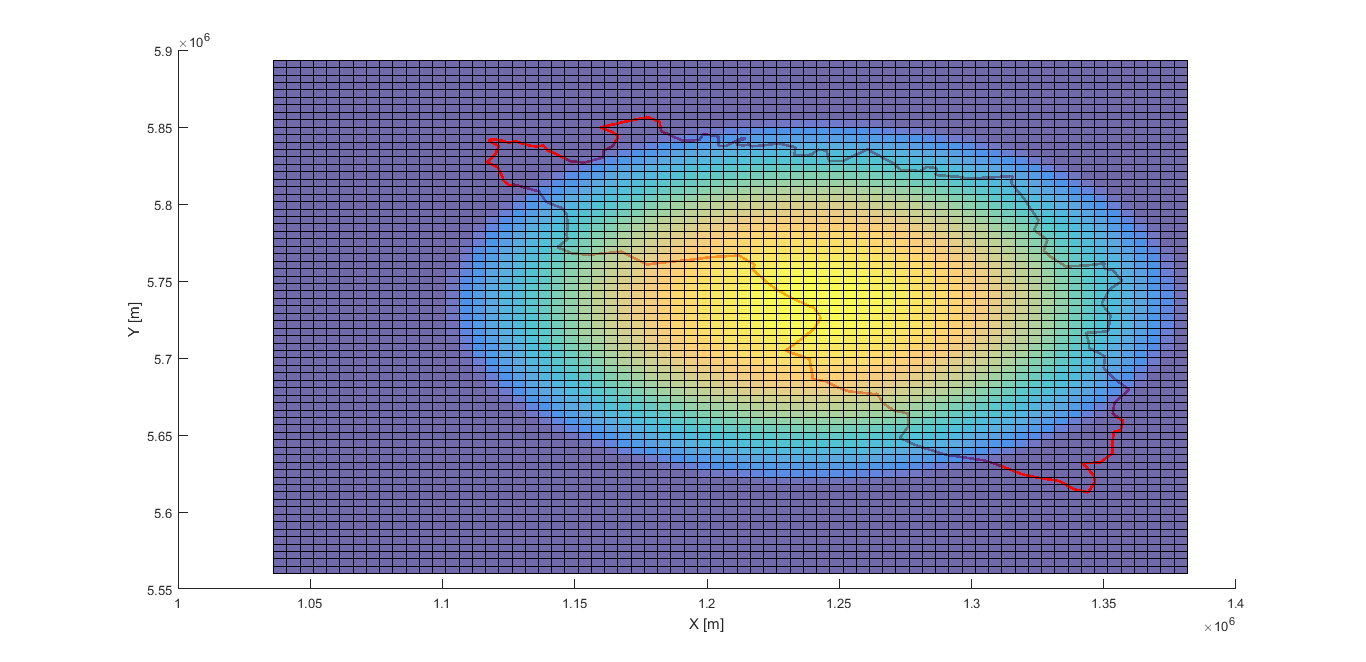
\includegraphics[width=1\linewidth]{chmura_paraboloidalna_2}
		\caption{Rzut wykresu.}
		\label{fig:parabola_2d}
	\end{subfigure}	

\label{fig:opad_paraboliczny}
\caption{Kształt funkcji opadu parabolicznego.}
\end{figure}

\begin{figure}[!ht]
	\label{fig:opad_wymierny}
	\begin{subfigure}{1\textwidth}
		\centering
		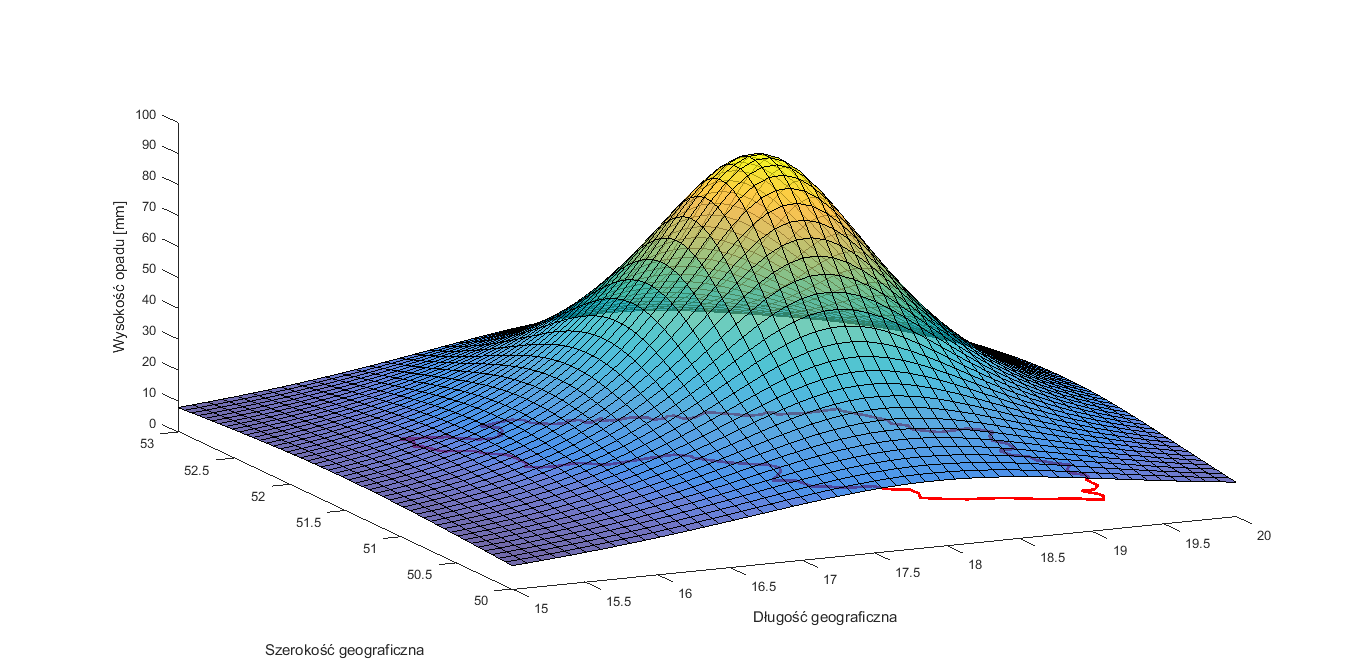
\includegraphics[width=1\linewidth]{chmura_wymierna_1}
		\caption{Wykres zastosowanej funkcji wymiernej}
		\label{fig:wymierna_3d}
	\end{subfigure}	
	\begin{subfigure}{1\textwidth}
		\centering
		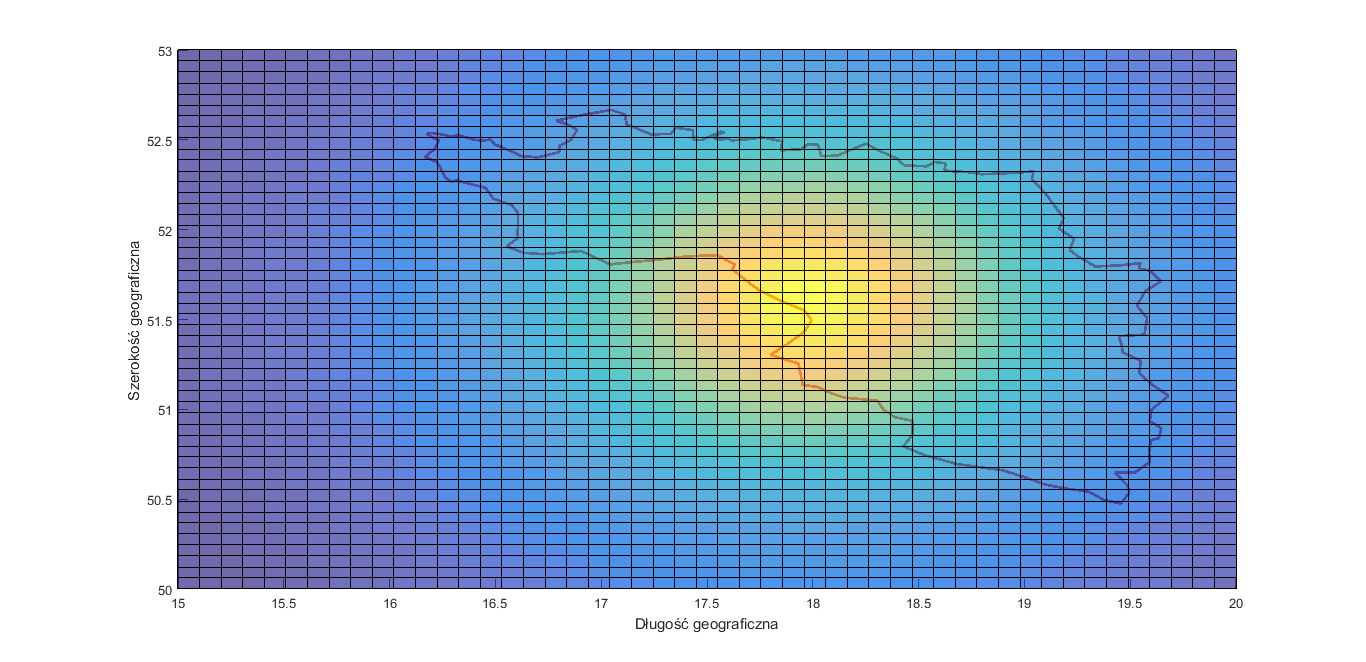
\includegraphics[width=1\linewidth]{chmura_wymierna_2}
		\caption{Rzut wykresu zastosowanej funkcji wymiernej}
		\label{fig:wymierna_2d}
	\end{subfigure}	
	\caption{Kształt funkcji opadu wymiernego.}
\end{figure}

Zdefiniowano również funkcję, która ma za zadanie wyznaczenie objętości rzeczywistego opadu we wskazanym trójkącie w~oparciu o~zadany wariant opadu. Zdecydowano się na numeryczne obliczanie całki podwójnej obszaru ograniczonego odcinkami trójkąta. Zrezygnowano z~podejścia analitycznego, ponieważ dla opadu parabolicznego z~użyciem sklejenia taki sposób jest niewygodny (konieczne byłoby zdefiniowanie funkcji ograniczającej obszar całkowania). Ponadto, w~przypadku niektórych testowanych funkcji (jak np. $e^{(x-x_0)^2 - (y-y_0)^2}$) nie ma możliwości analitycznego obliczenia całki\footnote{Kształt tej funkcji jest zbliżony do tej zdefiniowanej wzorem~\ref{eq:opad_wymierny}, dlatego pominięto go w~testach}, wobec tego użyta metoda numeryczna zachowuje uniwersalność oraz daje dowolną dokładność (co zostało wykazane eksperymentalnie). Tym sposobem zostało rozwiązane zagadnienie weryfikacji błędu działania algorytmu opisanego w~podrozdziale~\ref{sec:zastosowana_metoda}. Uzyskiwane wyniki porównywane są z~danymi pseudorzeczywistymi.



\section{Kroki implementacji}
W~ramach implementacji rozwiązania przygotowano zbiór punktów pełniących rolę posterunków opadowych oraz zestaw węzłów granicy obszaru, dla którego wyznaczony zostanie opad powierzchniowy.

Jak wspomniano na początku tego rozdziału, przeprowadzenie triangulacji oparto o~klasę \textit{delaunayTriangulation}~\cite{delaunayTriangulation}. Powstała siatka trójkątów została zaprezentowana na rysunku~\ref{fig:triagnulacja_danych}.

\begin{figure}[!ht]
	\centering
\begin{subfigure}{1\textwidth}
	\centering
	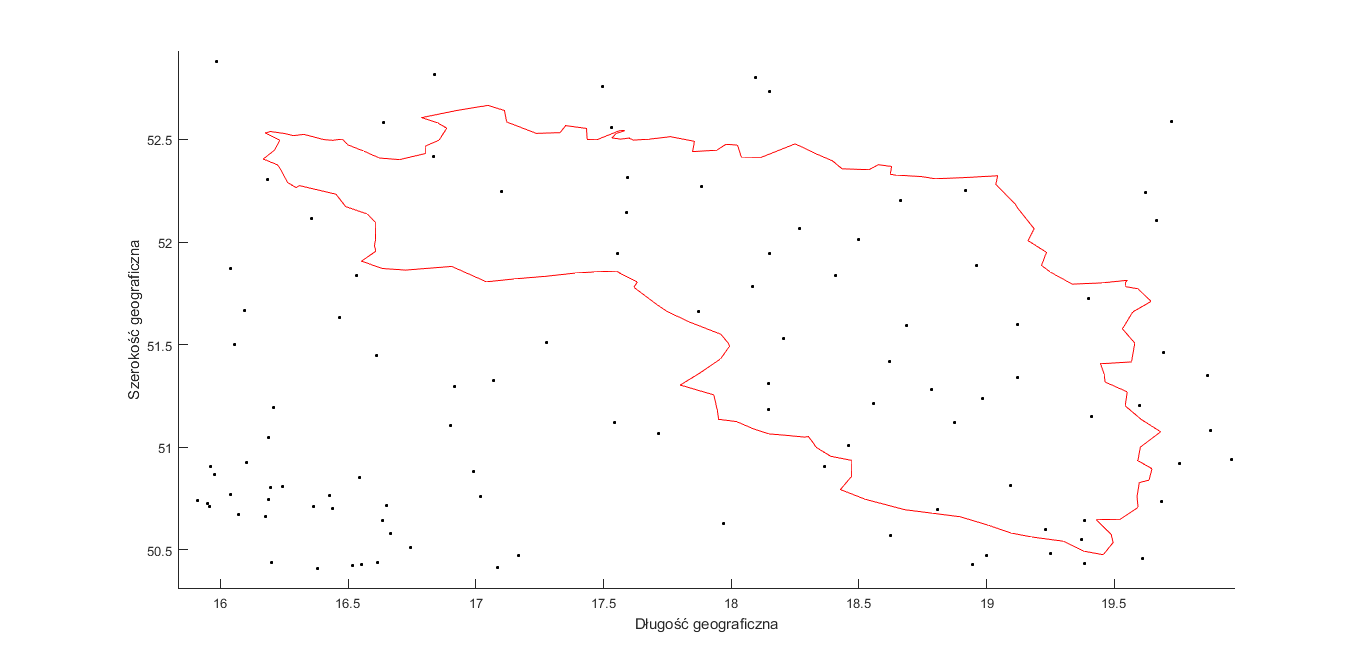
\includegraphics[width=1\linewidth]{dane_wejsciowe}
	\caption{Posterunki opadowe i~obszar zlewni}
	\label{fig:dane_wejsciowe}
\end{subfigure}	
	\begin{subfigure}{1\textwidth}
	\centering
	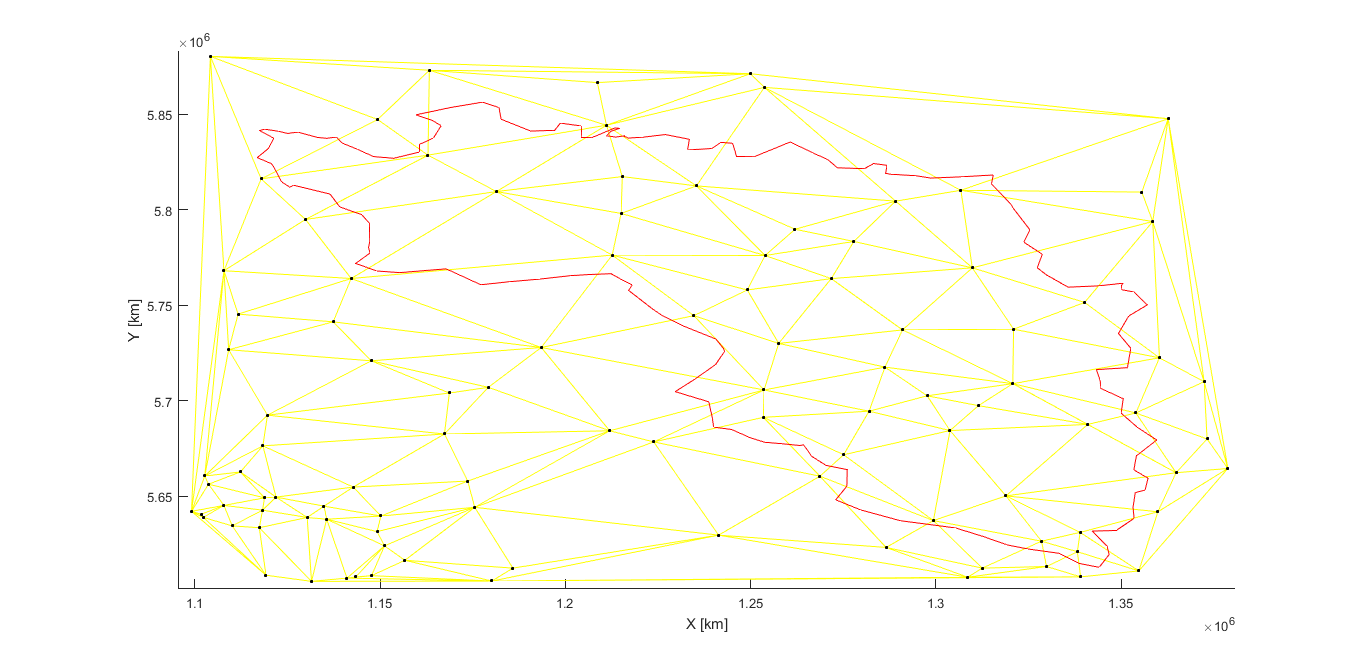
\includegraphics[width=1\linewidth]{triangulacja_zlewnia}
	\caption{Siatka triangulacji dla posterunków}
	\label{fig:triagnulacja_danych}
\end{subfigure}	
\caption{Prezentacja danych wejściowych}
	
\end{figure}


\begin{figure}[!ht]
	\centering
	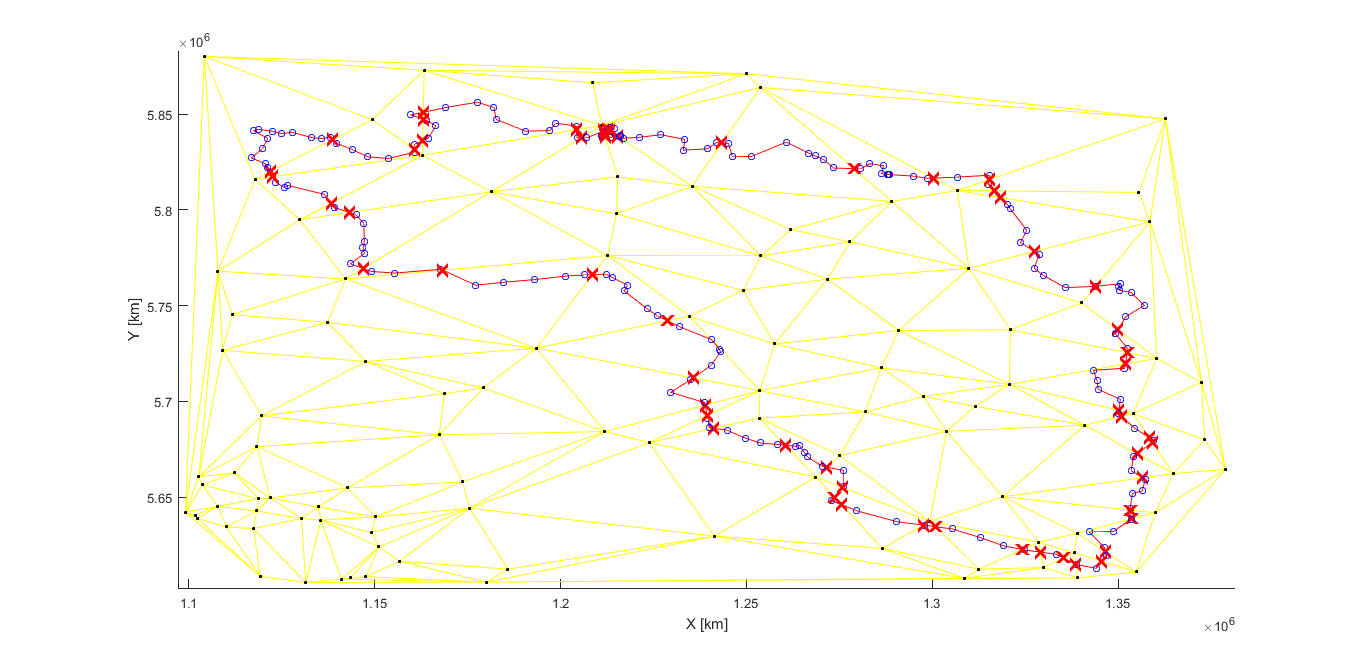
\includegraphics[width=1\linewidth]{punkty_do_interpolacji}
	\caption{Punkty wyznaczone do interpolacji.
	O - węzły granicy, X - przecięcia granicy z~liniami siatki.}
	\label{fig:punkty_interpolacji}
\end{figure}

Wyznaczenie wartości dla powstałych punktów odbywa się poprzez interpolację powierzchniową poszczególnych trójkątów. Stworzono mechanizm wyznaczający wektory normalne dla wygenerowanych trójkątów. 

Przy użyciu przygotowanej funkcji (opartej na wzorze~\ref{eq:wartosc_interpolowana}, dla wszystkich wyznaczonych do interpolacji punktów uzyskiwana jest wartość opadu korzystając ze współrzędnych $x$~i~$y$ punktu i~wektora normalnego trójkąta, w~którym ten punkt się znajduje.

\begin{figure}[!ht]
	\centering
	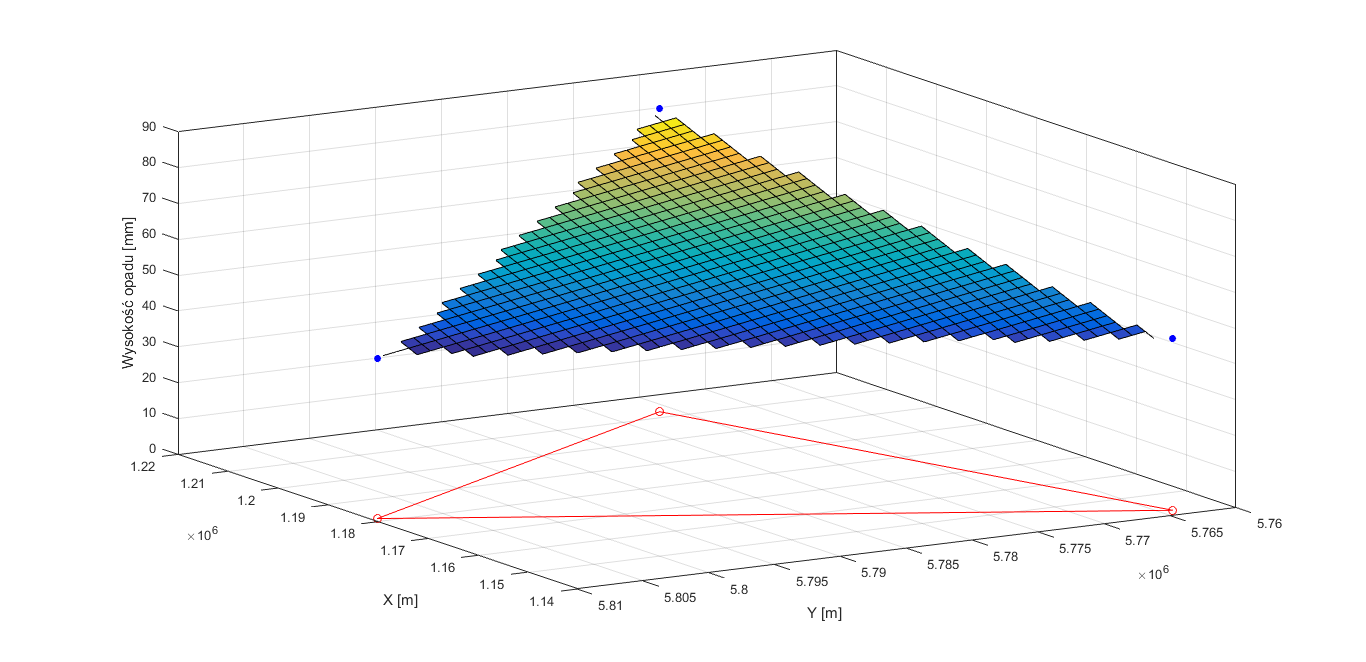
\includegraphics[width=1\linewidth]{prezentacja_interpolacji}
	\caption{Interpolacja płaszczyzną dla pojedynczego trójkąta.}
	\label{fig:plaszczyzna_interpolacji}
\end{figure}


Wyizolowane punkty, krytyczne z~punktu widzenia zadanego obszaru opadu, stanowią węzły kolejnej triangulacji. Jak zaprezentowano na rysunku~\ref{fig:druga_triangulacja}, pojawia się komplikacja wynikająca z~łączenia ze sobą wszystkich pobliskich punktów. Tym sposobem kreowane są trójkąty, które nie wprowadzają informacji dla rozwiązania. Co więcej, wpływają negatywnie na ewentualny wynik.

\begin{figure}[!ht]
	\centering
\begin{subfigure}{1\textwidth}
	\centering
	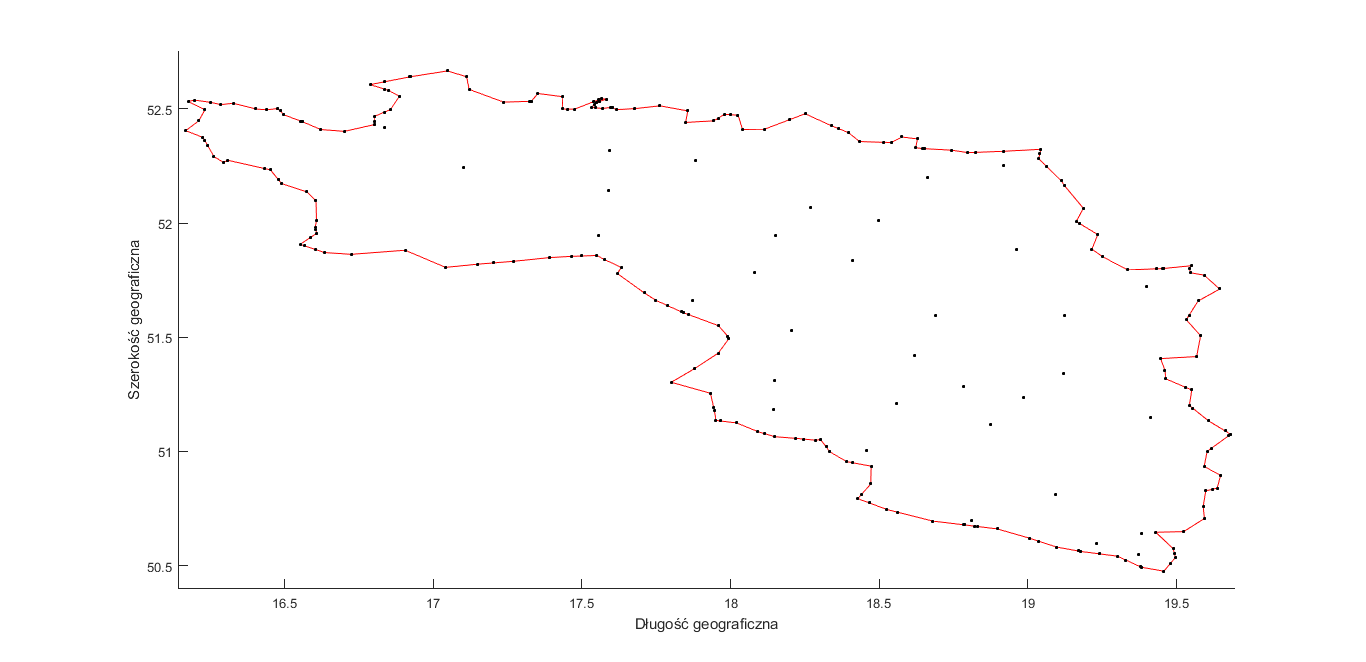
\includegraphics[width=1\linewidth]{dane_druga_triangulacja}
	\caption{Punkty dla ponownej triangulacji}
	\label{fig:dane_druga_triangulacja}
\end{subfigure}	
	\begin{subfigure}{1\textwidth}
	\centering
	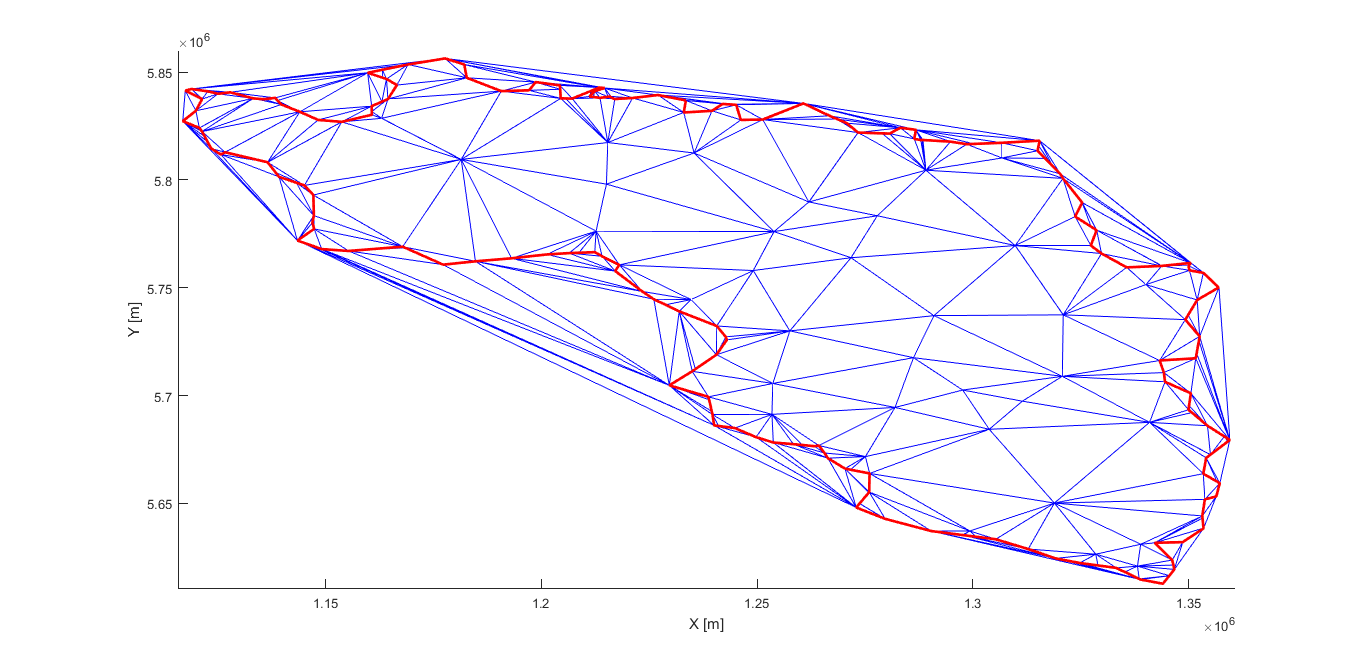
\includegraphics[width=1\linewidth]{druga_triangulacja}
	\caption{Siatka triangulacji dla wyznaczonych punktów}
\label{fig:druga_triangulacja}	
\end{subfigure}	
\caption{Triangulacja danych interpolowanych}
\end{figure}

Problem ten rozwiązano poprzez dodanie ograniczenia dla obiektu klasy \textit{delaunayTriangulation} zdefiniowanego jako zbiór węzłów triangulacji stanowiących granicę zlewni poddawanej analizie. Odfiltrowanie nieistotnych fragmentów wykonano stosując metodę \textit{isInterior}, która wskazuje czy poszczególne trójkąty utworzonej siatki zawierają się w~obszarze wskazanym przez ograniczenie. Rezultat tych kroków prezentuje rysunek~\ref{fig:druga_triangulacja_ograniczenie}

\begin{figure}[!ht]
	\centering
	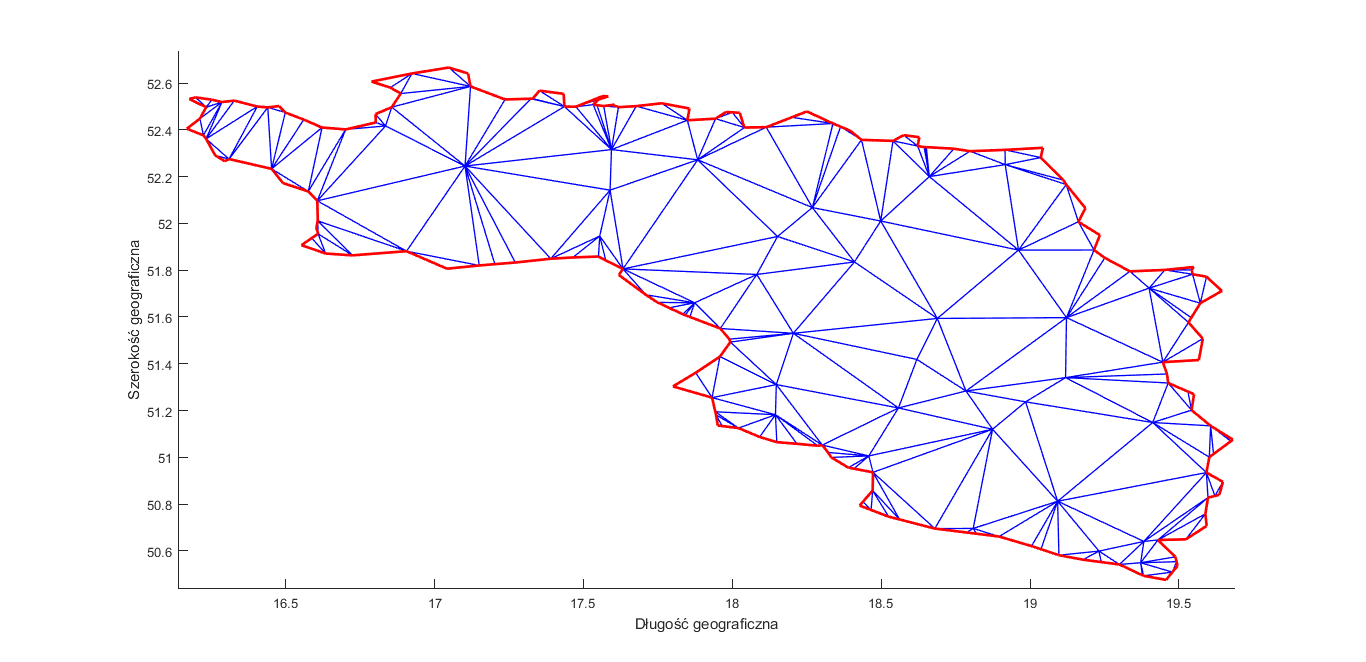
\includegraphics[width=1\linewidth]{druga_triangulacja_z_ograniczeniem}
	\caption{Triangulacja z~ograniczeniem obszarem zlewni}
	\label{fig:druga_triangulacja_ograniczenie}
\end{figure}

Ostatecznie, dla uzyskanych trójkątów wyznaczana jest wartość opadu powierzchniowego, co po zsumowaniu jest łącznym opadem na wskazanej zlewni.